%%%%%%%%%%%%%%%%%%%%%%%%%%%%%%%%%%%%%%%%%%%%%%%%%%%%%%%%%%%%%%%%%%%%%%%%%%%%%%%%
% AMS Beamer series / Bologna FC / Template
% Andrea Omicini
% Alma Mater Studiorum - Università di Bologna
% mailto:andrea.omicini@unibo.it
%%%%%%%%%%%%%%%%%%%%%%%%%%%%%%%%%%%%%%%%%%%%%%%%%%%%%%%%%%%%%%%%%%%%%%%%%%%%%%%%
%\documentclass[handout]{beamer}\mode<handout>{\usetheme{default}}
%
\documentclass[presentation, 8pt]{beamer}\mode<presentation>{\usetheme{AMSBolognaFC}}
%\documentclass[handout]{beamer}\mode<handout>{\usetheme{AMSBolognaFC}}
%%%%%%%%%%%%%%%%%%%%%%%%%%%%%%%%%%%%%%%%%%%%%%%%%%%%%%%%%%%%%%%%%%%%%%%%%%%%%%%%
\usepackage[T1]{fontenc}
\usepackage{wasysym}
\usepackage{amsmath,blkarray}
\usepackage{soul}
\usepackage[minted,most]{tcolorbox}
\usepackage{centernot}
\usepackage{fontawesome}
\usepackage{fancyvrb}
\usepackage{minted}
\usepackage{hyperref}
\usepackage{multicol}
\setminted[scala]{fontsize=\small,baselinestretch=1,obeytabs=true, tabsize=2}
\setminted[yaml]{fontsize=\large,frame=lines,linenos,baselinestretch=1,obeytabs=true, tabsize=2}
\usepackage[ddmmyyyy]{datetime}
\setminted{fontsize=\footnotesize}
\renewcommand{\dateseparator}{}
%\renewcommand{\thefootnote}{\fnsymbol{footnote}}
\newcommand{\version}{1}
\usepackage[
	backend=biber,
	citestyle=authoryear-icomp,
	maxcitenames=1,
	bibstyle=numeric]{biblatex}

	\makeatletter

\addbibresource{biblio.bib}
%%%%%%%%%%%%%%%%%%%%%%%%%%%%%%%%%%%%%%%%%%%%%%%%%%%%%%%%%%%%%%%%%%%%%%%%%%%%%%%%
\title[Programming with ScaFi!]
{Programming (and Learning) Self-Adaptive \& Self-Organising Behaviour with ScaFi}
\subtitle{for Swarms, Edge-Cloud Ecosystems, and More}
%
%
\author[\sspeaker{Casedei}]
{\speaker{Roberto Casadei} \href{mailto:roby.casadei@unibo.it}{roby.casadei@unibo.it} \\
\speaker{Gianluca Aguzzi} \href{mailto:gianluca.aguzzi@unibo.it}{gianluca.aguzzi@unibo.it} \\
\speaker{Danilo Pianini} \href{mailto:danilo.pianini@unibo.it}{danilo.pianini@unibo.it} \\
\speaker{Mirko Viroli} \href{mailto:mirko.viroli@unibo.it}{mirko.viroli@unibo.it}}
%
\institute[DISI, Univ.\ Bologna]
{%Dipartimento di Informatica -- Scienza e Ingegneria (DISI)\\
\textsc{Alma Mater Studiorum} -- Universit{\`a} di Bologna \\[0.1cm]
\textbf{Talk @} \bold{International Conference on Autonomic Computing and Self-Organizing Systems (ACSOS)}\\[0.15cm]

\includegraphics[width=0.15\textwidth]{img/qr-code-scafi.png}

\includegraphics[width=0.15\textwidth]{img/qr-code.png}
}
%
\renewcommand{\dateseparator}{/}
\date[\today]{\today}
%
\AtBeginSubsection[]
{
  \begin{frame}
  \frametitle{Contents}
  \tableofcontents[currentsubsection, 
	sectionstyle=show/shaded, 
	subsectionstyle=show/shaded]
  \end{frame}
}
\AtBeginSection[]
{
  \begin{frame}
  \frametitle{Contents}
  \tableofcontents[currentsubsection, 
	sectionstyle=show/shaded, 
	subsectionstyle=show/shaded]
  \end{frame}
}
%%%%%%%%%%%%%%%%%%%%%%%%%%%%%%%%%%%%%%%%%%%%%%%%%%%%%%%%%%%%%%%%%%%%%%%%%%%%%%%%
\begin{document}
%%%%%%%%%%%%%%%%%%%%%%%%%%%%%%%%%%%%%%%%%%%%%%%%%%%%%%%%%%%%%%%%%%%%%%%%%%%%%%%%
\frame{\titlepage}
%===============================================================================
\section{Introduction}
%%%%%%%%%%%%%%%%%%%%%%%%%%%%%%%%%%%%%%%%%%%%%%%%%%%%%%%%%%%%%%%%%%%%%%%%%%%
\subsection{Context -- Collective Adaptive Systems}
\begin{frame}{Context}
\begin{exampleblock}{Modern IT systems are more and more \bold{complex}}
	\begin{itemize}
		\item incresing availability of werable/mobile/embedded/flyings devices
		\item increasing availability of heterogeneous wireless networks
		\item increasing availability of computational resources (edge/fog/cloud computing)
		\item increasing production of data \bold{everywhere} and \bold{anytime}
	\end{itemize}
\end{exampleblock}
\begin{alertblock}{The challenge}
	Consider the worst case possible scenario
	\begin{itemize}
		\item \bold{zillion} of devices \emph{unpredictably} locaed and moving in a space
		\item heterogeneous displacement, \bold{pervasive} sensing/actuation
		\item computational services are \bold{contextual} (proximity-based) and \emph{dynamic} 
	\end{itemize}
\end{alertblock}
\begin{center}
\Large{How can we \bold{program} such systems?}
\end{center}
\begin{center}
	\Large{What are the right \bold{abstractions}?}
	\end{center}
\end{frame}
\begin{frame}[plain,c]
	\begin{center}
	{\Huge \textbf{Collective Adaptive Systems} (CASs)}\\
	{\large Systems composed of \emph{possibly} \bold{large} set of component executing a \bold{collective} task strongly relying on component \bold{interactions} and showing \bold{inherent} \emph{adaptivity}.}\\[0.3cm]
	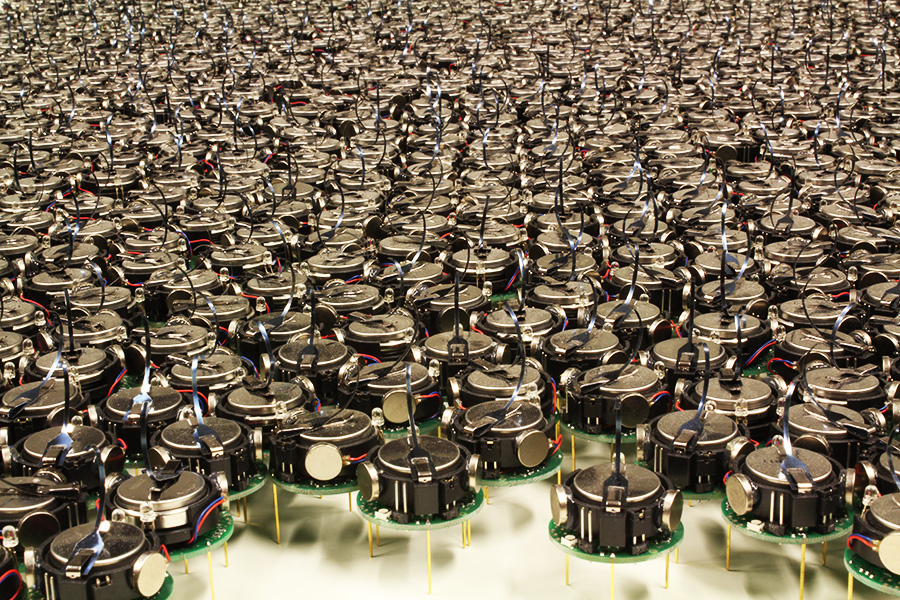
\includegraphics[width=0.28\textwidth]{img/swarms.jpg}
	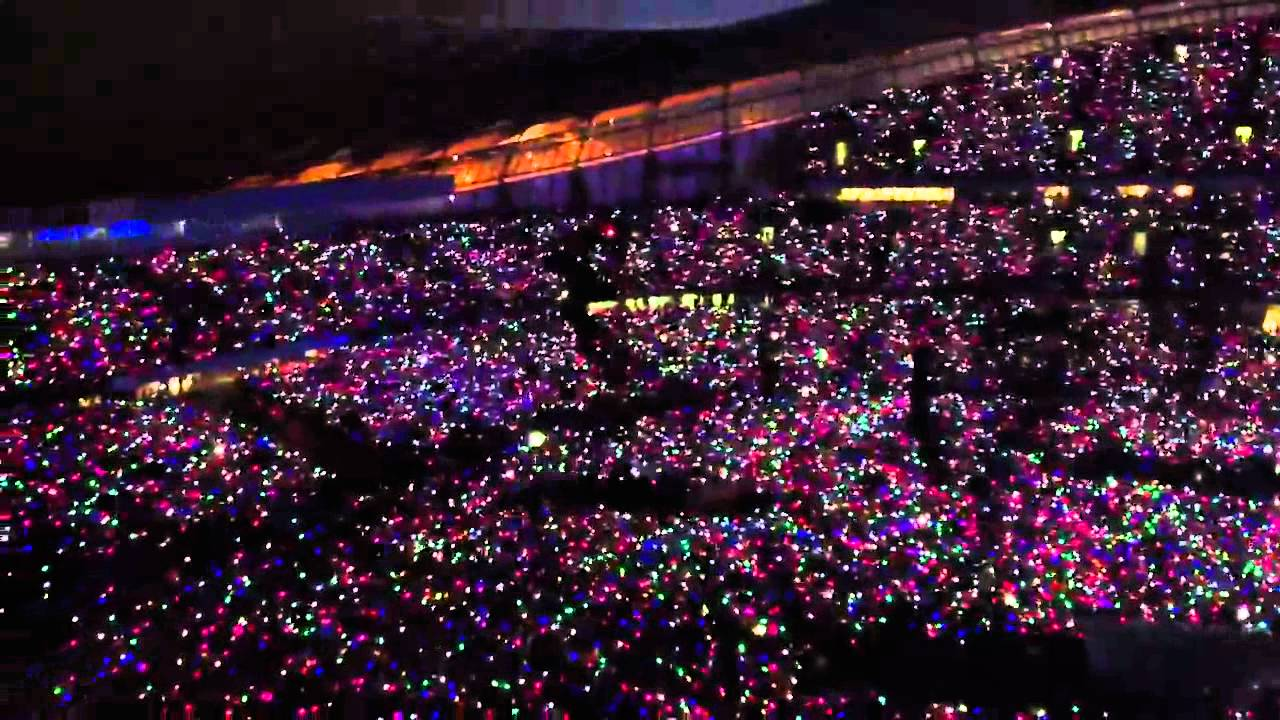
\includegraphics[width=0.333\textwidth]{img/coldplay.jpg}
	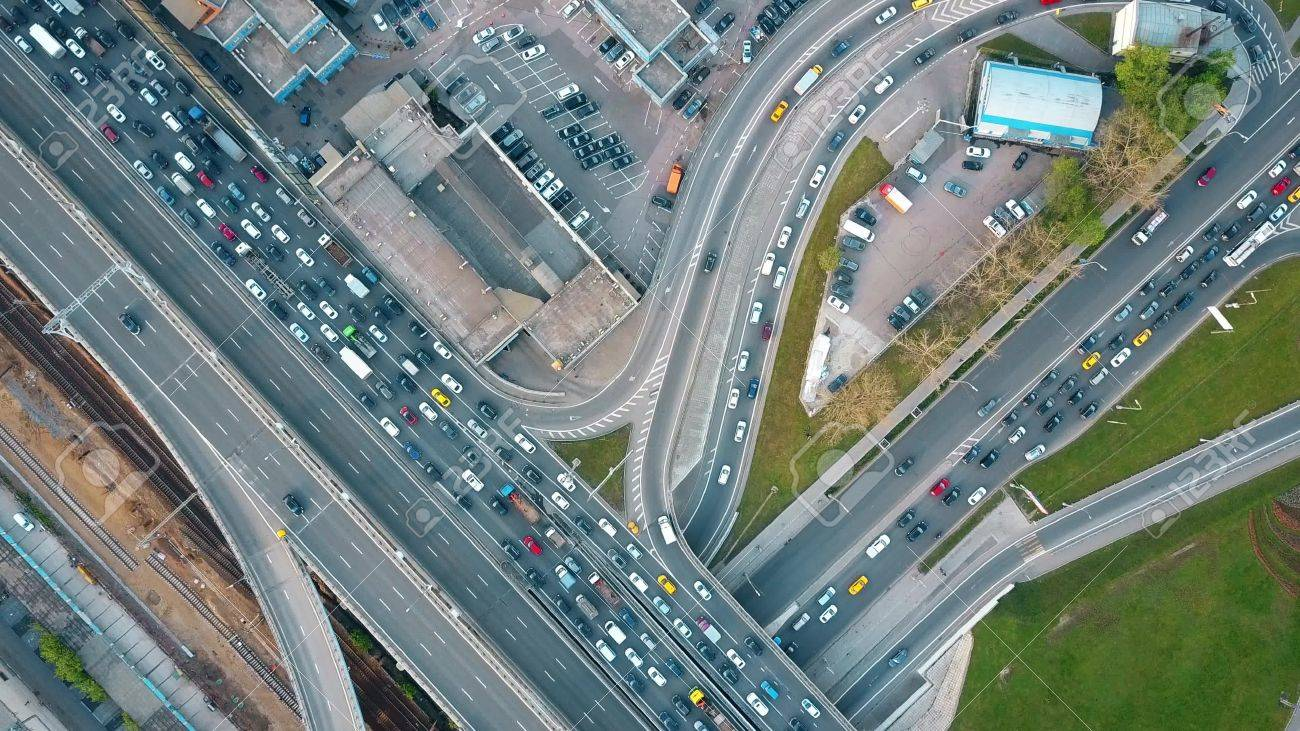
\includegraphics[width=0.333\textwidth]{img/traffic.jpg}	
	\end{center}
\end{frame}
\begin{frame}{Examples: controlling a fleets of drones}
\centering
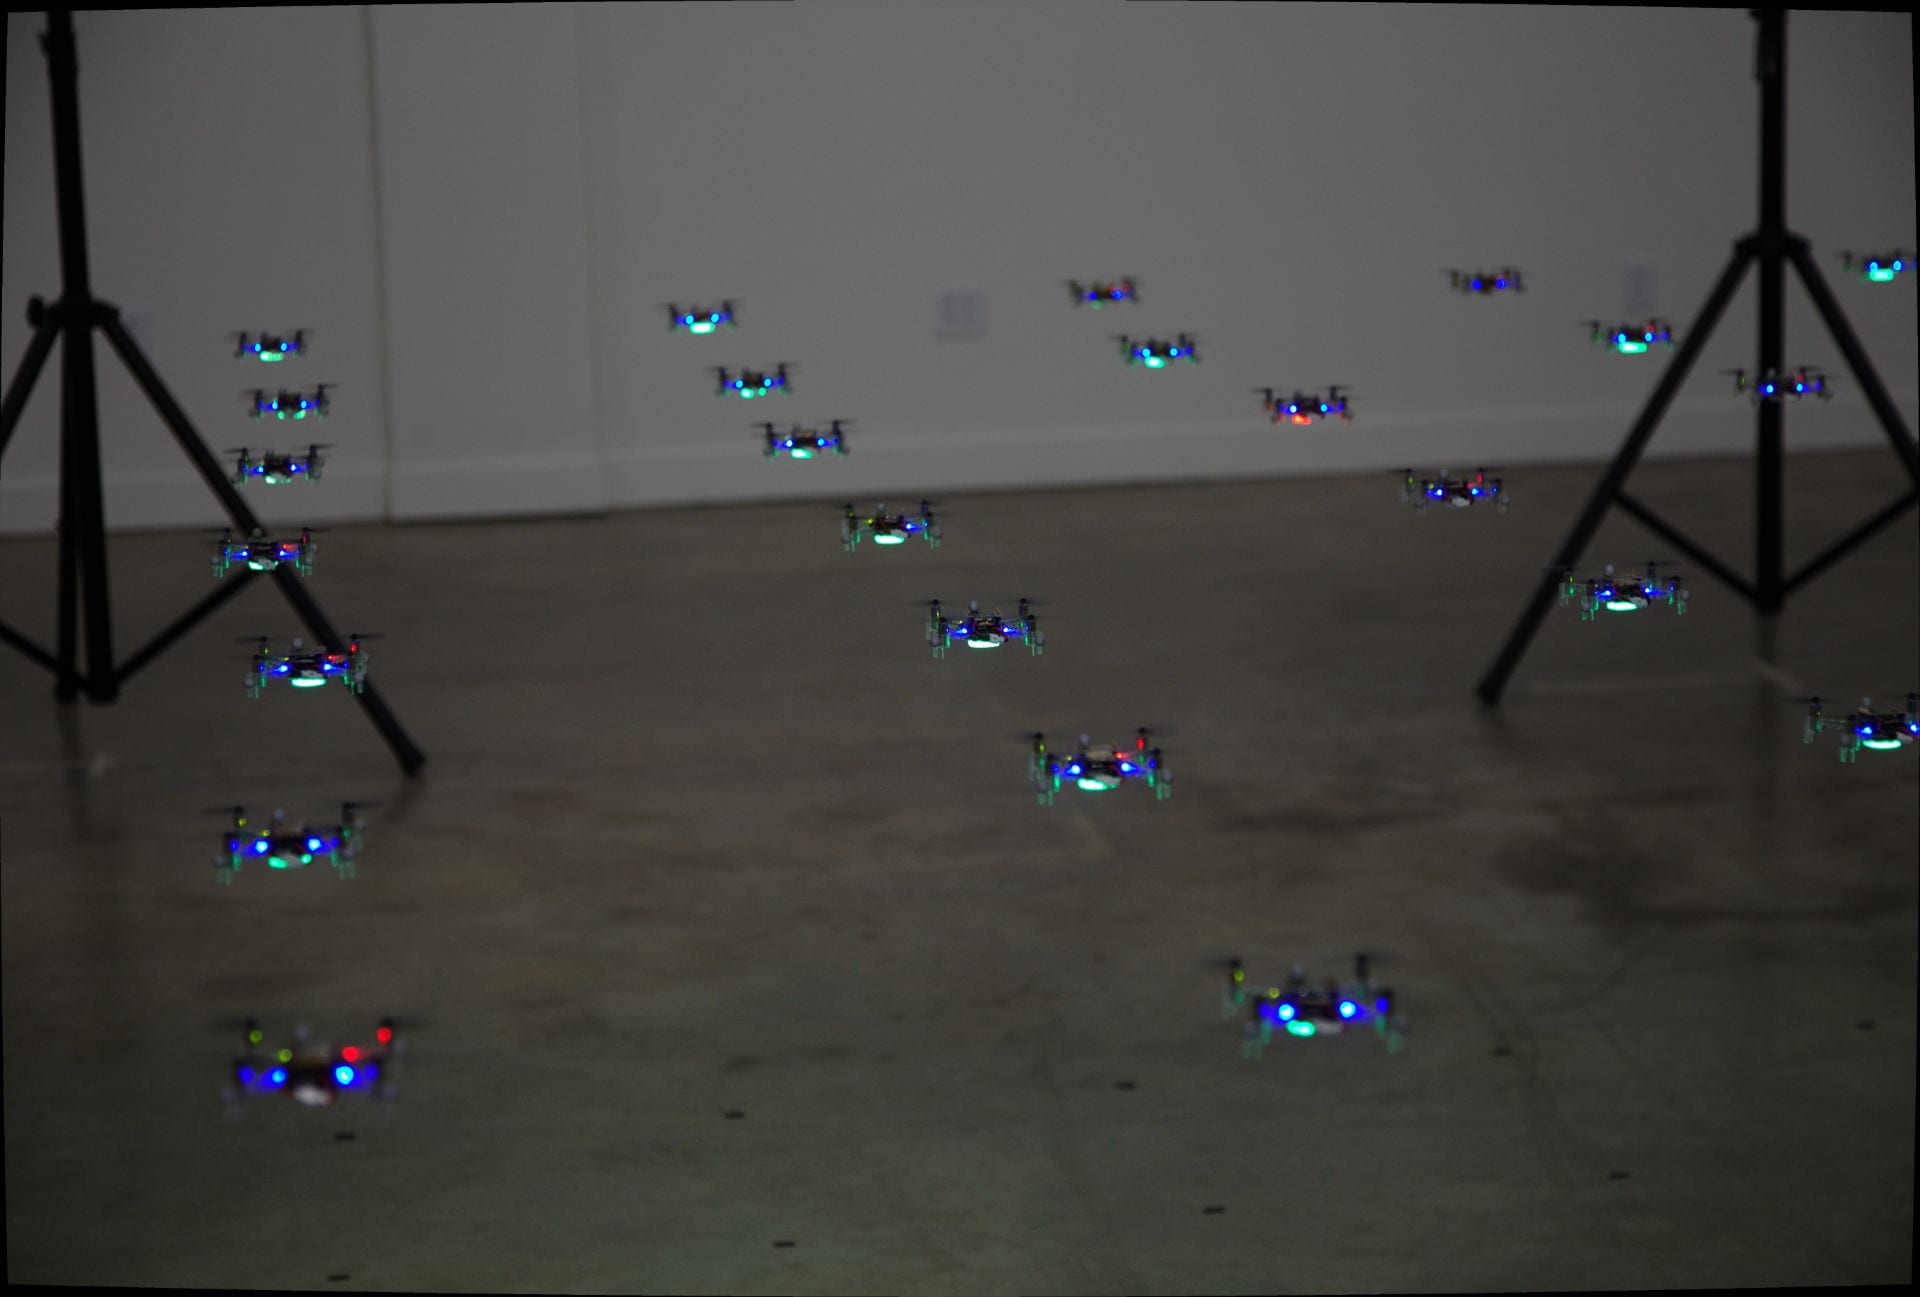
\includegraphics[width=0.7\textwidth]{img/crazyflies}
\begin{alertblock}{Issues}
\begin{itemize}
	\item Design techniques to \bold{reactively} propagate information across the fleet
	\item Create algorithms for \bold{higher-level} programming of the fleet
\end{itemize}
\end{alertblock}
\end{frame}
\begin{frame}{Examples: pedestrian steering in (smart)cities}
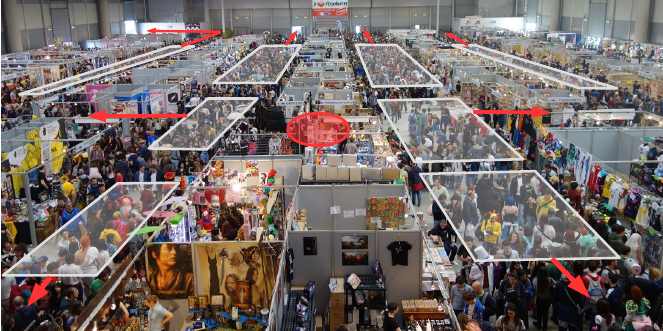
\includegraphics[width=0.9\textwidth]{img/pedastrian.png}
\begin{alertblock}{Issue}
	\begin{itemize}
		\item Design \bold{self-organisation} algorithms for people navigation
		\item More generally, design map-based large scale applications
	\end{itemize}
\end{alertblock}
\end{frame}
\begin{frame}{Examples: fine control of crowds}
\centering
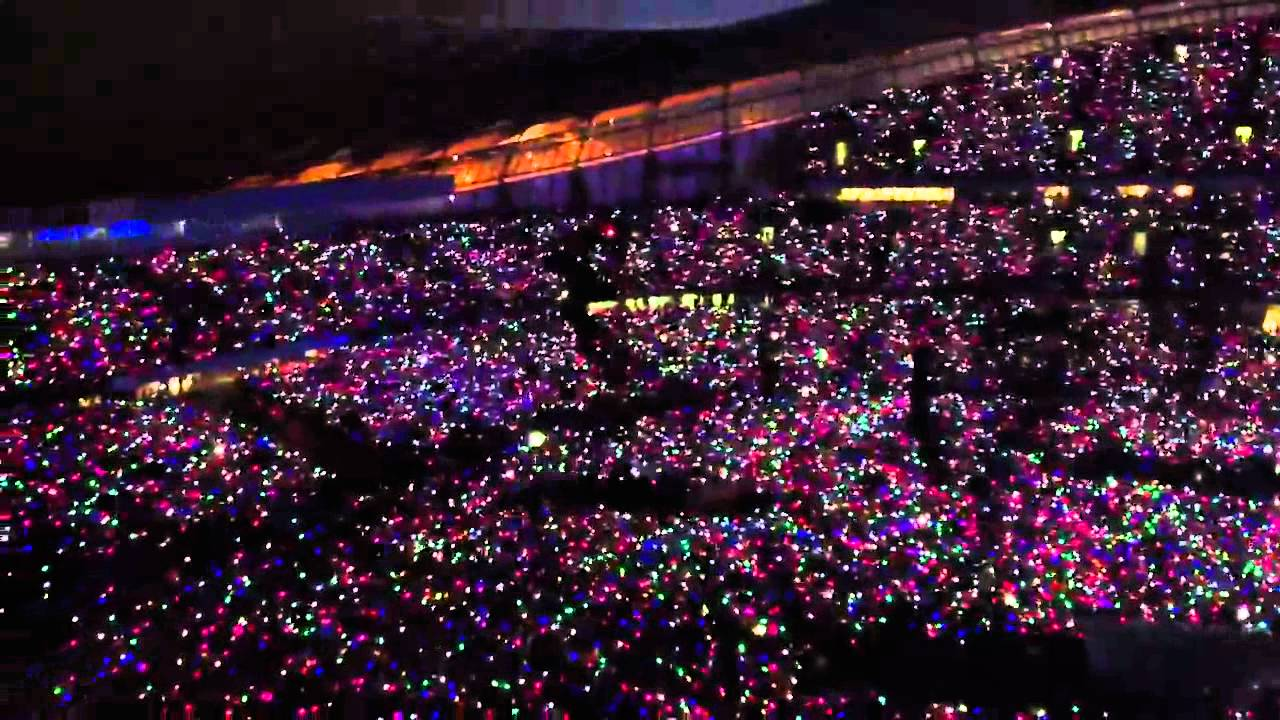
\includegraphics[width=0.9\textwidth]{img/coldplay}
\begin{alertblock}{Issues}
	\begin{itemize}
		\item Evaluating the influence of environment in crowd formation
		\item Evaluating the influence of ambient sensors, cameras and wearable
		devices
	\end{itemize}
\end{alertblock}
\end{frame}
\begin{frame}{Collective \underline{Adaptive} Systems}
\begin{alertblock}{\textbf{Adaptation}}
A system is \emph{adaptive} if it is able to \bold{change} its own behaviour
depending on \bold{circumstances}, in order to better reach its \emph{goal}\\
\faArrowRight \, Adaptivess in \bold{intrisic} to open complex system (like CASs)
\end{alertblock}
\begin{exampleblock}{Kind of adaptiveness, self-* properties}
	\centering
	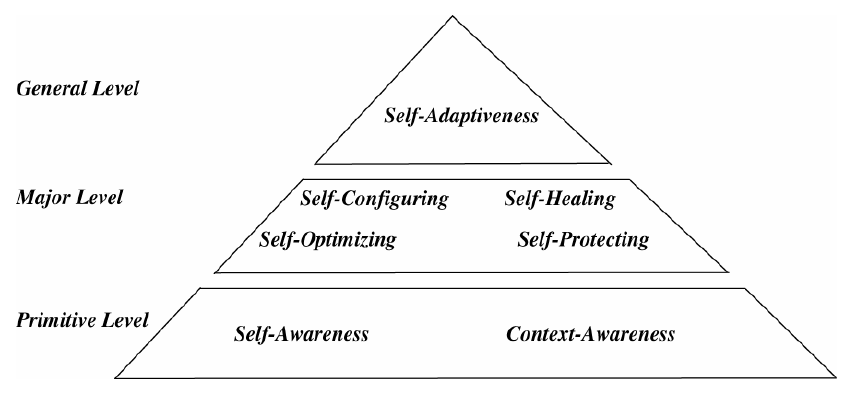
\includegraphics[width=0.8\textwidth]{img/self-*.png}
\end{exampleblock}
\end{frame}
\begin{frame}{Kind of adaptiveness}
\begin{exampleblock}{Self-adaptiveness: general level}
	\begin{itemize}
		\item \bold{self-adaptiveness} \faArrowRight \, the ultimate property we perceive from outside
		\item the terms ``self-*'' recalls a property achieved in \bold{autonomy}
		\item subcases: self-managing, -governing, -maintenance, -control
	\end{itemize}
\end{exampleblock}
\begin{exampleblock}{Major level}
	\begin{itemize}
		\item internal properties related to overall system management
		\item subcases: self-configuring, self-healing, self-optimising, self-protecting
		\item defined in the context of \bold{autonomic} computing
	\end{itemize}
\end{exampleblock}
\begin{exampleblock}{Primitive level}
	\begin{itemize}
		\item internal properties related to primitive aspects
		\item subcases: self-awareness, context-awareness
		\item means being able to properly perceive the own state, context, \dots
	\end{itemize}
\end{exampleblock}
\end{frame}
\begin{frame}{The case of self-organisation}
\begin{alertblock}{Self-organisation}
	\centering
	The ability of creating \bold{spatial/temporal} patterns out of the \emph{local interaction} of individuals
\end{alertblock}
\begin{exampleblock}{Self-adaptive vs. self-organising}
\begin{itemize}
	\item self-adaptive: a top-down way of achieving adaptiveness
	\item[\faArrowRight] we have the adaptation goal, and accordingly guide components 
	\item self-organising: a bottom-up way of achieving adaptiveness
	\item[\faArrowRight] the adaptive behaviour emerges from local interactions
	\begin{itemize}
		\item The typical approach in large scale CASs
		\item Born in the context of \bold{swarm intelligence}
	\end{itemize}
\end{itemize}
\end{exampleblock}
\end{frame}
%%%%%%%%%%%%%%%%%%%%%%%%%%%%%%%%%%%%%%%%%%%%%%%%%%%%%%%%%%%%%%%%%%%%%%%%%%%%%%%
\begin{frame}{Good Abstraction for CASs?}
\begin{alertblock}{Ideas}
	\begin{itemize}
		\item specify \bold{overall} behaviour, not \emph{individual} device program
		\item abstract from the actual shape of \bold{interactions}
		\item \bold{automatically} adapt to environment details
		\item focus on how the \bold{global output} pattern can be obtained from global inputs
		\item focus on both \bold{spatial} and \bold{temporal} computing patterns
		\item[\faArrowRight] the ideas around macro-programming paradigms!
		\begin{itemize}
			\item \bold{Aggregate computing}
			\item Buzz
			\item \dots
		\end{itemize}
		\item Ruccurent abstractions:
		\begin{itemize}
			\item Ensembles \& collective tasks
			\item Self-organising information flows
			\item Self-healing collective structures (e.g., \emph{gradients})
		\end{itemize}
	\end{itemize}
\end{alertblock}
\end{frame}
\subsection{Aggregate Computing}
\begin{frame}[c, plain]
\begin{center}
	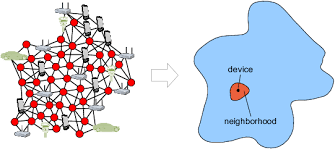
\includegraphics[width=0.5\textwidth]{img/aggregate-computing-structure.png}\\
	{\Huge \textbf{Aggregate Computing}}\\
	{\large Program the \bold{aggregate}, not the individual device} \\[0.2cm]
\end{center}
{\faCircle \, \normalsize{\emph{Computing Machine}} \faArrowRight \, an ensemble of devices as a single body, fading the actual space}\\
{\faCircle \, \normalsize{\emph{Elaboration process}} \faArrowRight \, atomic manipulation of a \emph{collective} data structure (\bold{computational field})}\\
{\faCircle \, \normalsize{\emph{Networked computation}} \faArrowRight \,
a proximity-based self-organising system hidden ``under-the-hood''}
\end{frame}
\begin{frame}{Computational model -- self-organising like execution}
\begin{itemize}
	\item \emph{Continuous} communication with \bold{neighbours} only (\faArrowRight decentralisation)
	\item \emph{Continous} execution of async \bold{rounds} of sense - compute - communicate
\end{itemize}
\centering
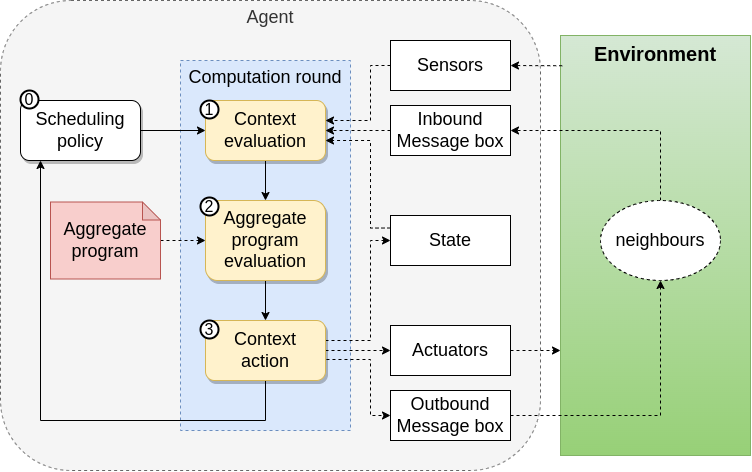
\includegraphics[width=0.8\textwidth]{img/execution-step.png}
\end{frame}
\begin{frame}[fragile]{Computational Fields: a static view}
	\begin{alertblock}{Traditionally a map: \textit{Space} $\mapsto$ \textit{Values}}
		\begin{itemize}
			\item possibly: evolving over time, dynamically injected, stabilising
			\item smoothly adapting to very heterogeneous domains
			\item more easily \emph{``understood''} on continuous and flat spatial domains
			\item ranging to booleans, reals, vectors, functions
		\end{itemize}
	\end{alertblock}
	\vfill
	\begin{multicols}{3}
		{\fbox{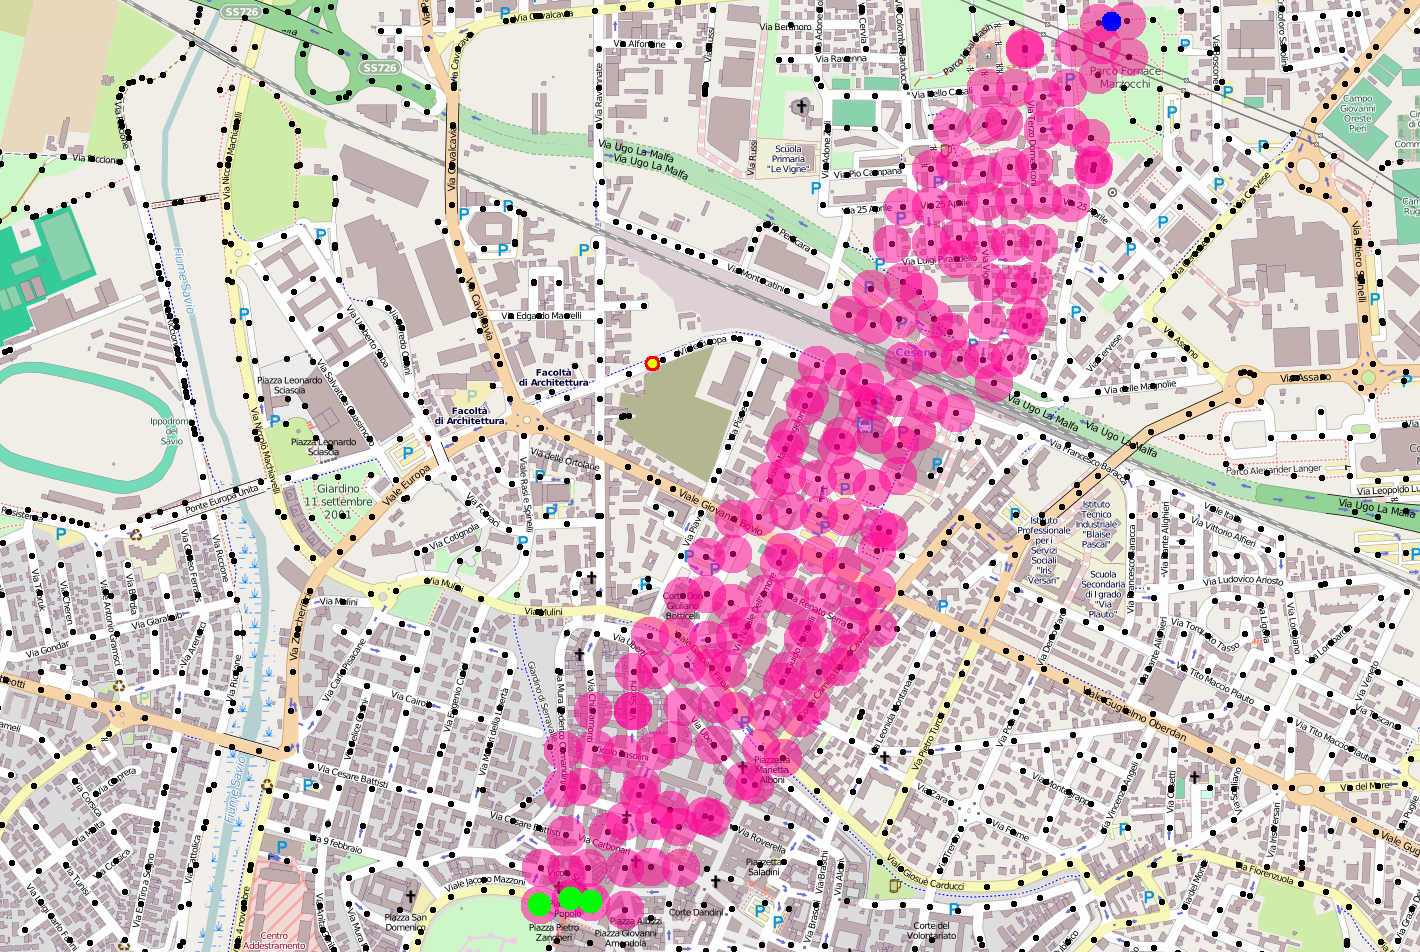
\includegraphics[height=2.3cm]{img/cesena0.png}} boolean channel in 2D}
		{\fbox{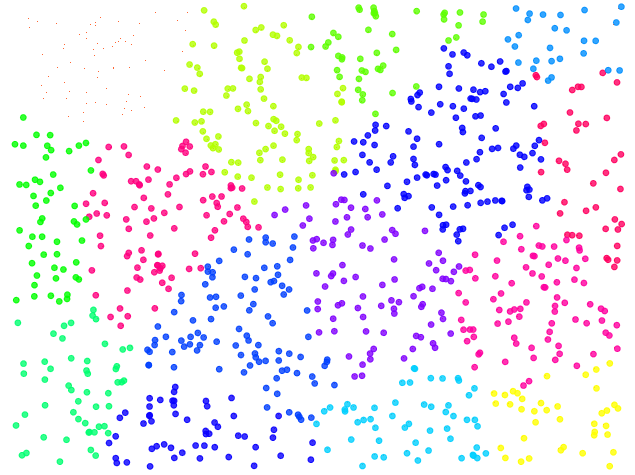
\includegraphics[height=2.3cm]{img/partition.png}} numeric partition in 2D}
		{\fbox{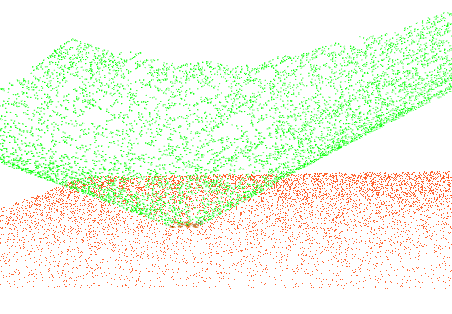
\includegraphics[height=2.3cm]{img/surface2.png}} real-valued gradient in 3D}
	\end{multicols}
\end{frame}
\begin{frame}{Computational Fields revisited: a dynamic view}
\begin{alertblock}{A field as a \textit{space-time} structure: $\phi:D\mapsto V$}
\begin{itemize}
		\item {\it event} $E$: a triple $\langle \delta, t, p\rangle$ -- device $\delta$, ``firing'' at time $t$ in position $p$
		\item {\it events domain} $D$: a coherent set of events (devices cannot move too fast)
		\item {\it field values} $V$: any data value
		\item[\faArrowRight] computation abstracts from/adapts to the underlying event
		\item[\faArrowRight] scheduling of events is essentially exogenous
\end{itemize}
\end{alertblock}
\begin{center}
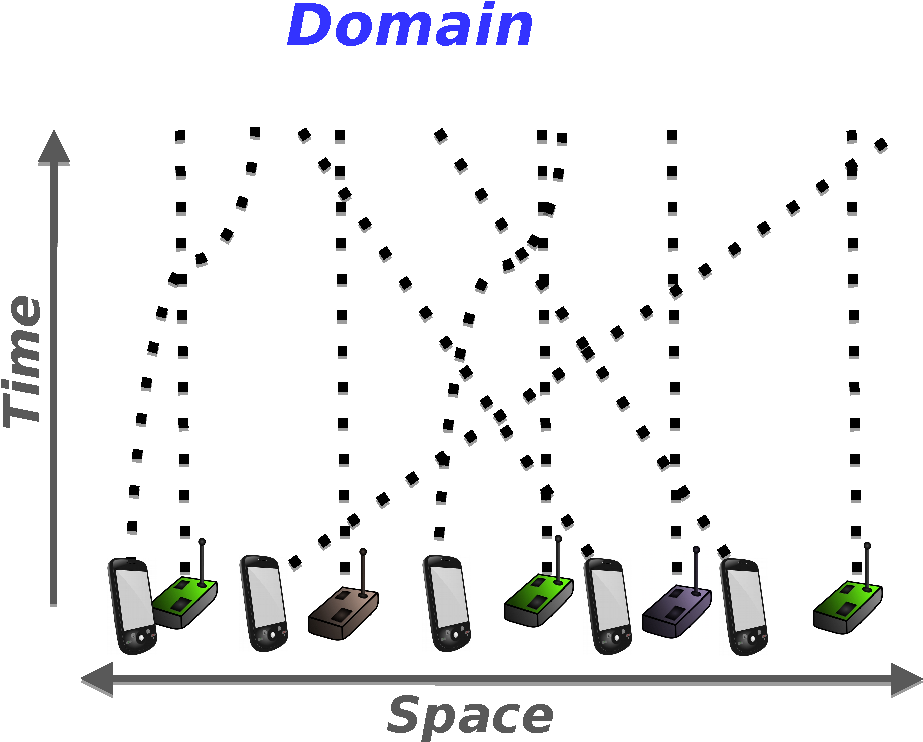
\includegraphics[height=4cm]{img/spacetime1.pdf}~~~~~~~~~~
\only<2->{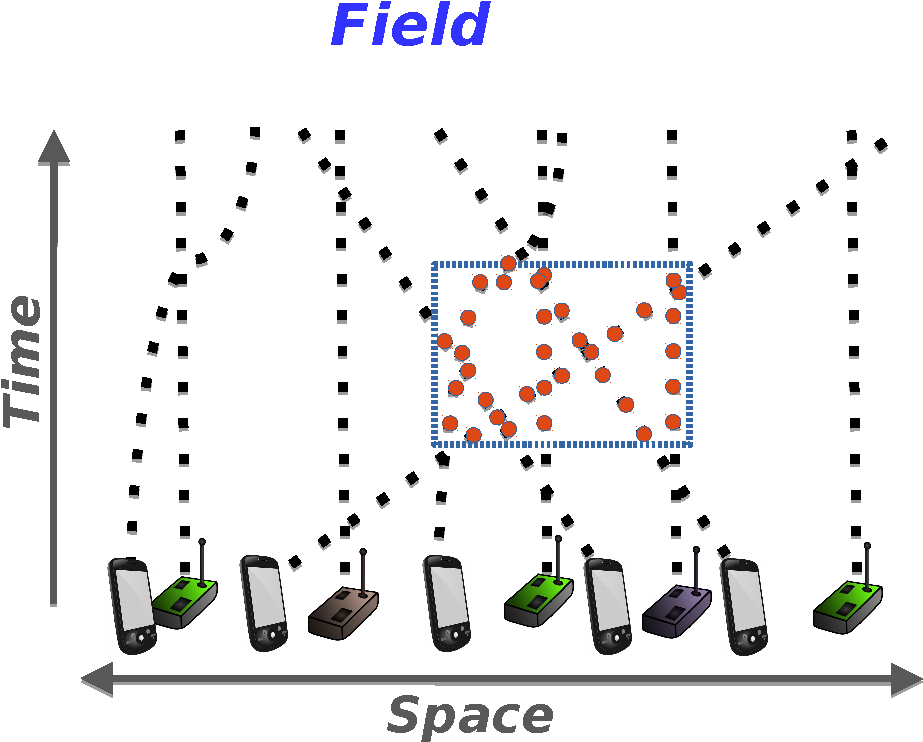
\includegraphics[height=4cm]{img/spacetime2.pdf}} 
\end{center}
\only<3->{will later show only snapshots of fields in 2D space..}
\end{frame}
\begin{frame}{Aggregate programming as a functional approach}
\begin{exampleblock}{Functionally composing fields}
\begin{itemize}
	\item Inputs: sensor fields, Output: actuator field
	\item Computation is a pure function over fields (time embeds state!)
	\item[\faArrowRight] for this to be practical/expressive we need a good programming language
\end{itemize}
\end{exampleblock}
\centering
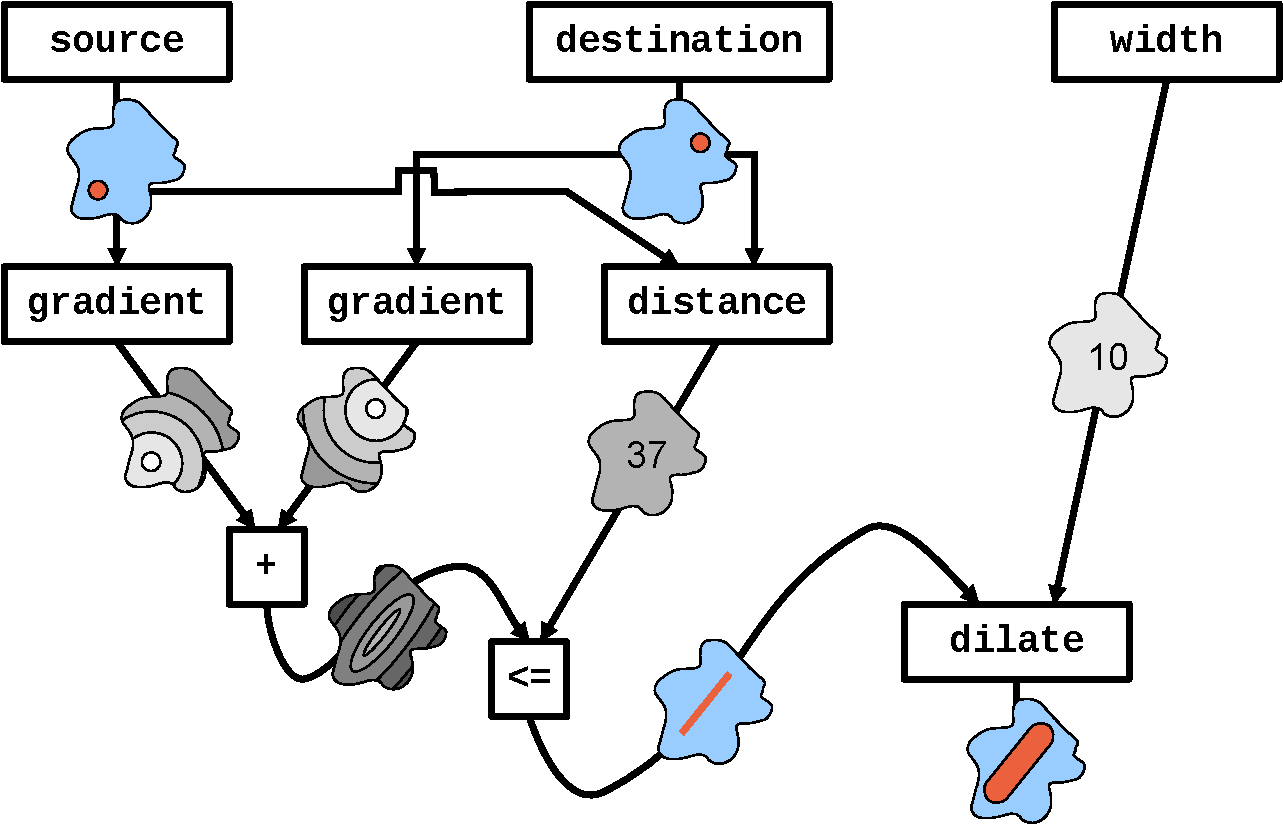
\includegraphics[width=0.65\textwidth]{img/functions.pdf}
\end{frame}
\begin{frame}[c, plain]
\begin{center}
	
\includegraphics[width=0.2\textwidth]{img/qr-code-scafi.png}\\
	{\Huge \textbf{ScaFi} (\bold{Sca}la \bold{Fi}elds)}\\
	{\large A Scala toolkit providing an \emph{internal domain-specific} language, \emph{libraries}, a \emph{simulation} environment, and \emph{runtime} support for \bold{practical} aggregate computing systems development} \\[0.3cm]
	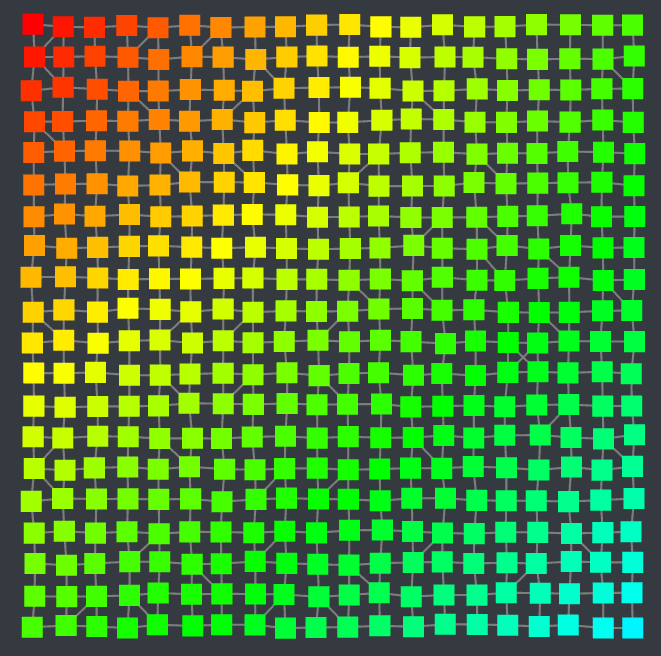
\includegraphics[width=0.2\textwidth]{img/gradient-scafi.png}
	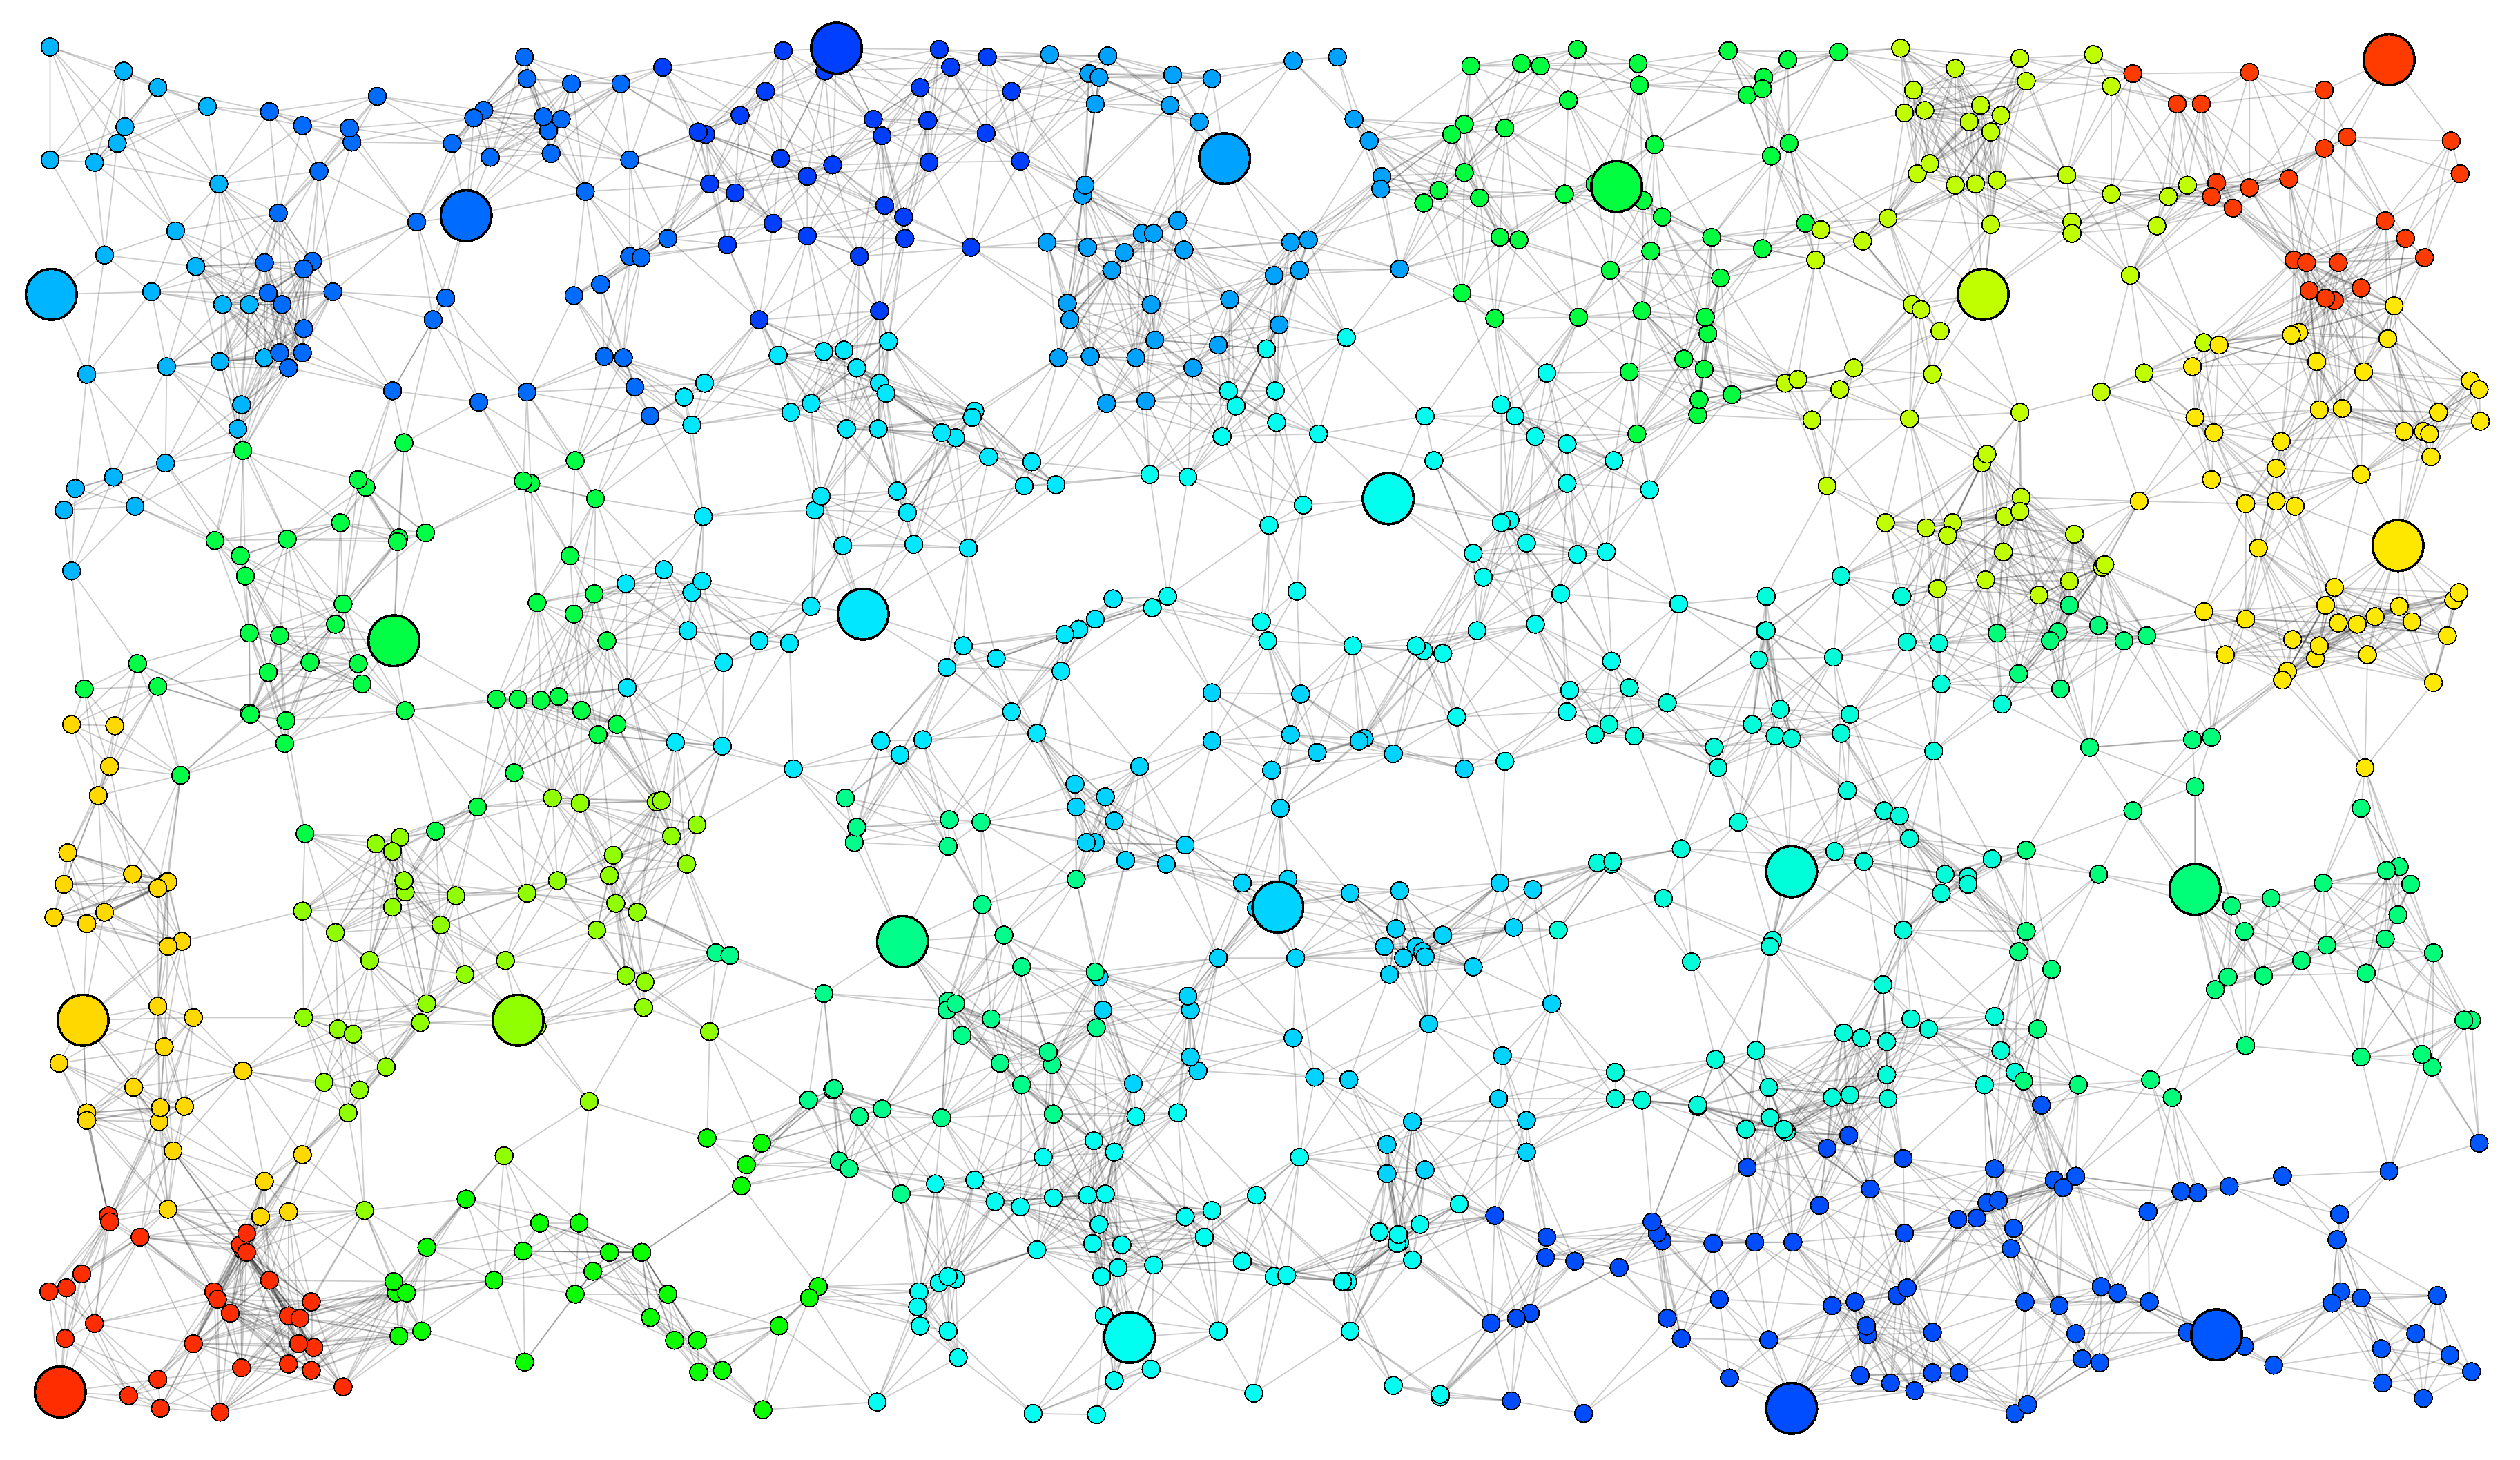
\includegraphics[width=0.35\textwidth]{img/scr-result.png}
	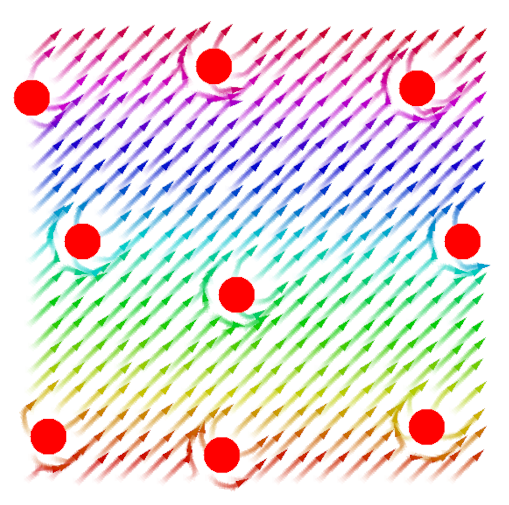
\includegraphics[width=0.215\textwidth]{img/obstacle-avoidance.png}
\end{center}
\end{frame}
%===============================================================================
\section{Playing with ScaFi!}%%%%%%%%%%%%%%%%%%%%%%%%%%%%%%%%%%%%%%%%%%%%%%%%%%%%%%%%%%%%%%%%%%%%%%%%%%%%%%%
\subsection{Guided Examples}
%%%%%%%%%%%%%%%%%%%%%%%%%%%%%%%%%%%%%%%%%%%%%%%%%%%%%%%%%%%%%%%%%%%%%%%%%%%%%%%
\subsection{Self-organising blocks -- Gradient and Channel}
%===============================================================================
\section{ScaFi in real-world scenarios: Integration with Alchemist}
\subsection{Alchemist}
\begin{frame}[c, plain]
\begin{center}
	
\includegraphics[width=0.2\textwidth]{img/qr-code.png}\\
	\Huge \textbf{Alchemist}\\
	{\large An \bold{extensible} \emph{meta}-simulator for \textbf{pervasive} computing scenarios}\\[0.3cm]
	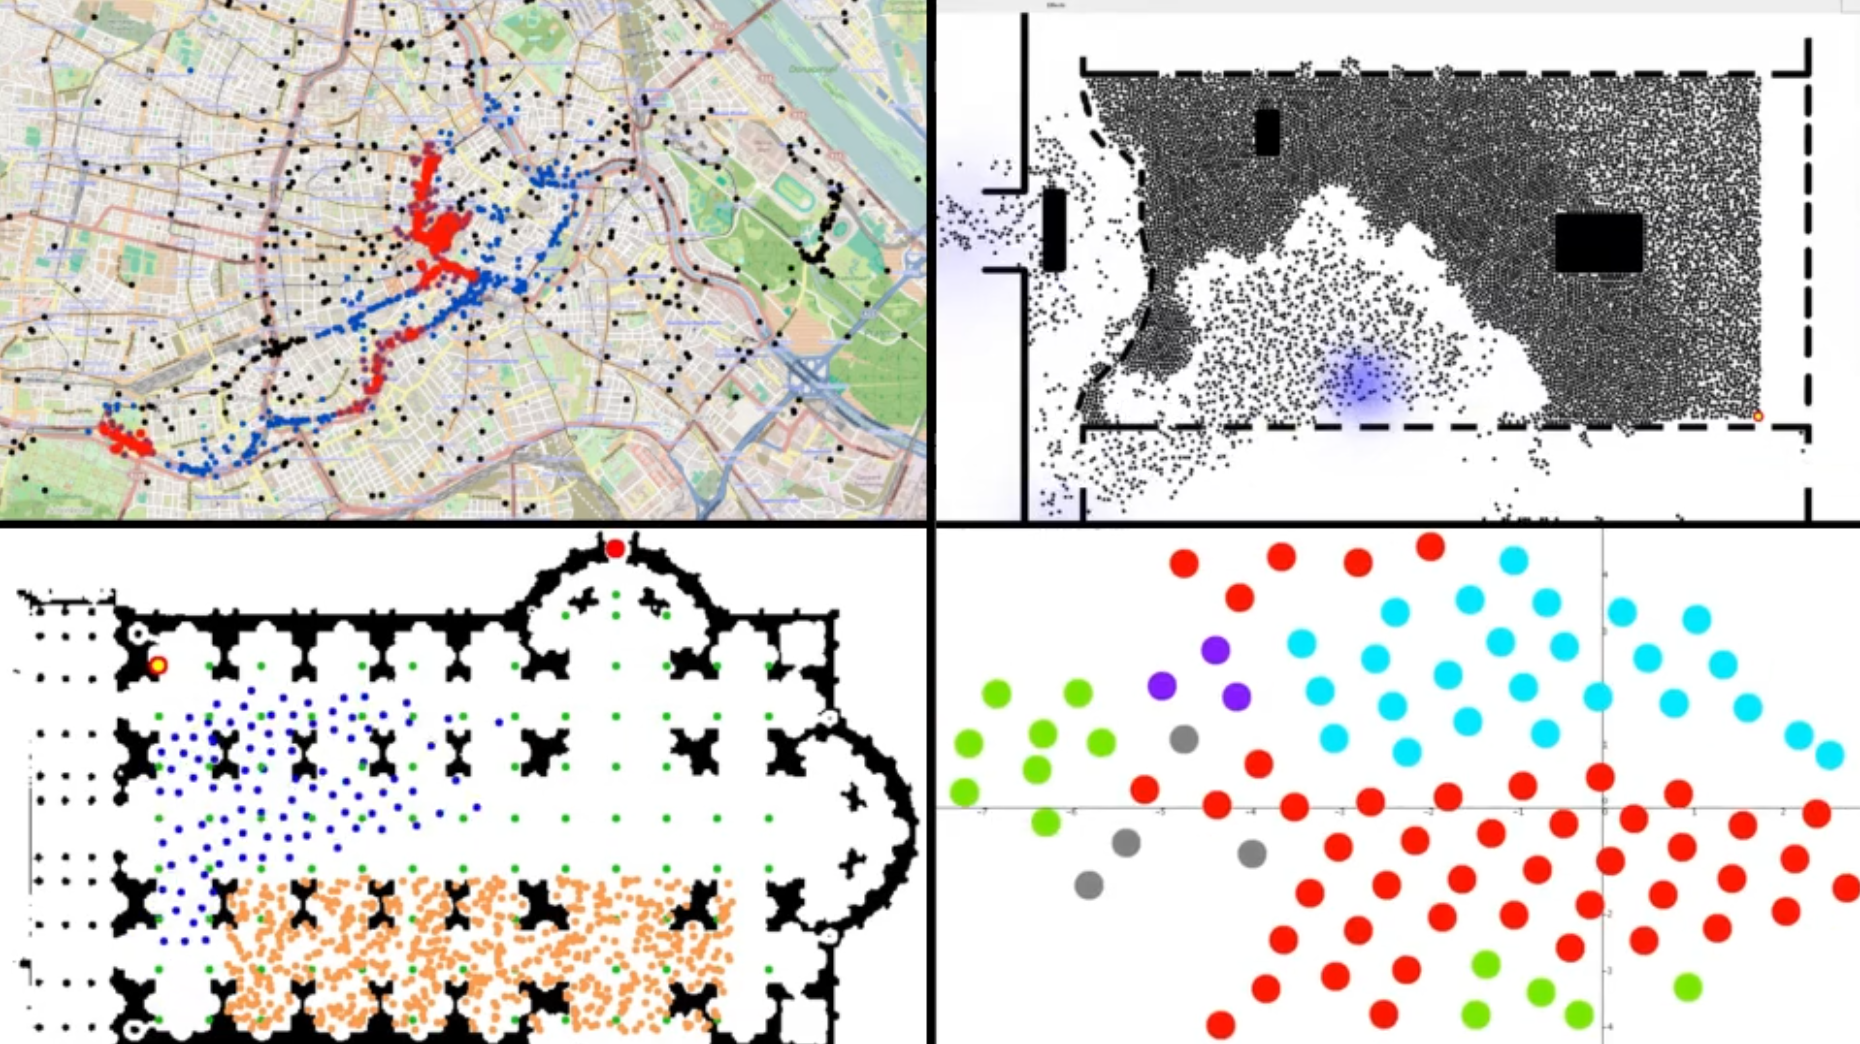
\includegraphics[width=0.5\textwidth]{img/alchemist-recap.png}
\end{center}
\end{frame}
\begin{frame}{Abstract model}
\centering
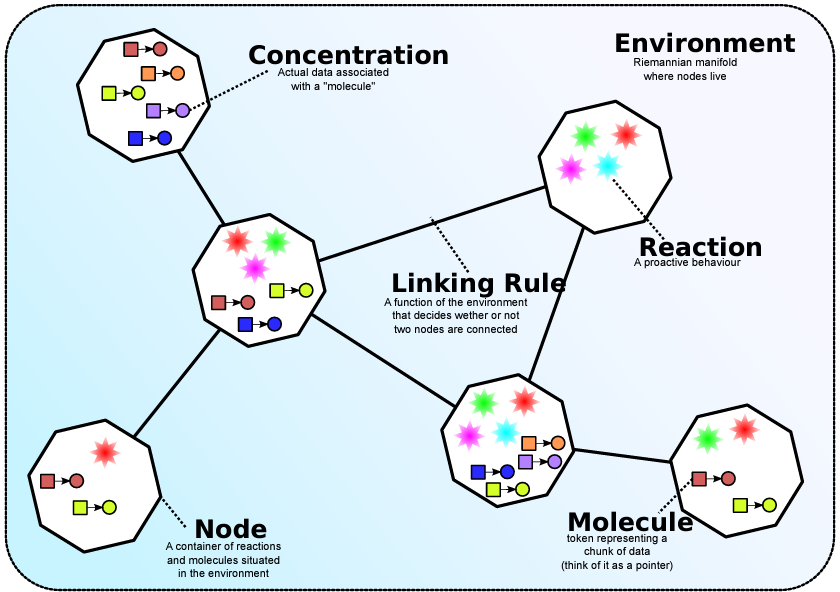
\includegraphics[width=0.8\textwidth]{img/abstract-model.png}
\end{frame}
\begin{frame}{Reactions}
\centering
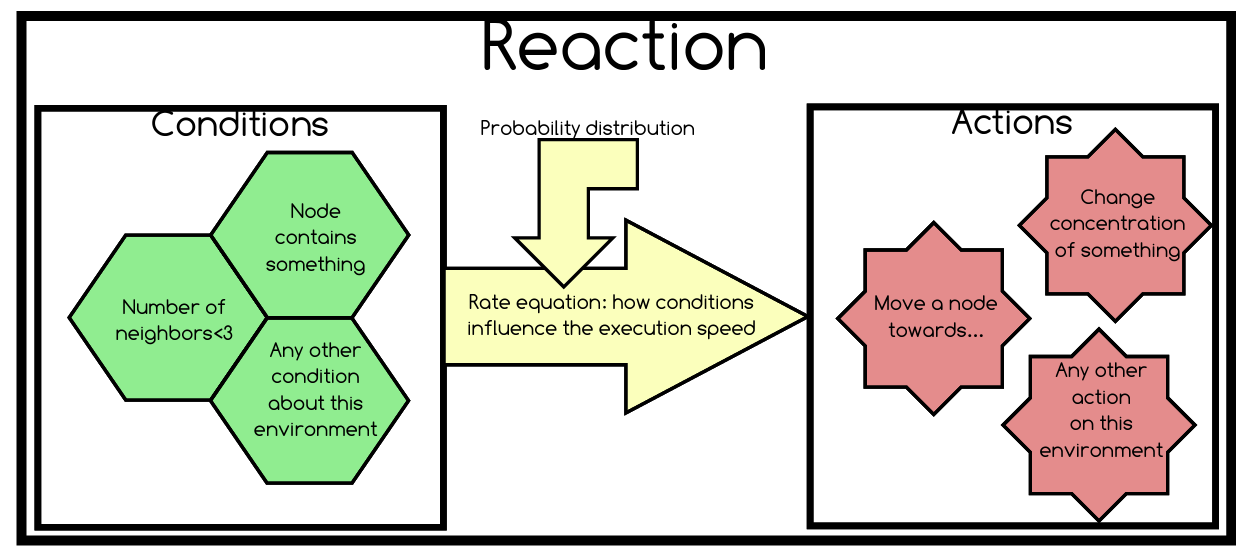
\includegraphics[width=0.8\textwidth]{img/reaction-model.png}
\end{frame}
\begin{frame}{Overall Architecture}
\centering
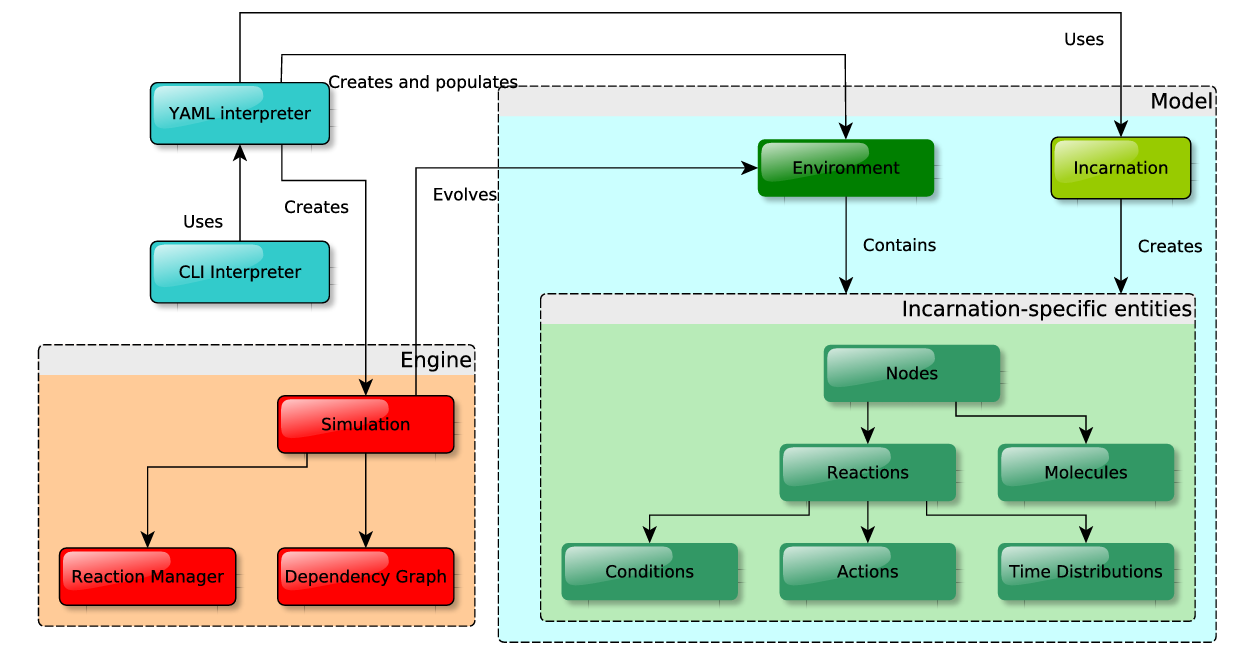
\includegraphics[width=0.8\textwidth]{img/alchemist-architecture.png}
\end{frame}
\begin{frame}{ScaFi Incarnation}
\begin{block}{Motivation}
	\begin{itemize}
		\item ScaFi has it own simulator \dots
		\item \dots but it is not as powerful as Alchemist, which:
		\begin{itemize}
			\item support GPS traces
			\item can simulate thousands of nodes
			\item can simulate different kinds of networks
			\item can simulate different mobility models
		\end{itemize}
	\end{itemize}
\end{block}
\begin{exampleblock}{ScaFi-Alchemist known uses}
	\begin{itemize}
		\item Swarm Robotics API: MacroSwarm\footnote[frame]{\fullcite{macroswarm}}
		\item Large-Scale smart cities simulations: FloodWatch\footnote[frame]{\fullcite{iee-floodwatch}}
		\item Crowd simulations
		\item \dots
	\end{itemize}
\end{exampleblock}
\end{frame}
\begin{frame}{Writing Simulations with ScaFi incarnation}
\begin{itemize}
	\item Alchemist uses YAML\footnote{\url{https://learnxinyminutes.com/docs/yaml/}} as language for writing simulations
	\begin{itemize}
		\item YAML is a human-readable data-serialization language
		\item It is a superset of JSON
		\item Support anchors and references
	\end{itemize}
	\item The same syntax is useds for \bold{any} incarnations
	\item Support running in \bold{batch}
	\item No compilation is needed 
	\begin{itemize}
		\item[\faThumbsUp] Once you have your ScaFi script compiled, you can run it in several alchemist simulations!!
	\end{itemize}
	\item Support ad-hoc export of simulation data through csv files. 
\end{itemize}
\end{frame}
\begin{frame}[fragile]{Minimal specification}
\begin{minted}{yaml}
incarnation: scafi
\end{minted}
\end{frame}
\begin{frame}[fragile]{Node displacement and connection}
\begin{minted}{yaml}
incarnation: scafi
network-model:
  type: ConnectWithinDistance
  parameters: [0.5]

# More deployments at 
# https://alchemistsimulator.github.io/howtos/simulation/deploy
deployments: # Description of where the nodes should be
  type: Grid
  parameters: [-5, -5, 5, 5, 0.25, 0.25, 0, 0]
\end{minted}
\end{frame}
\begin{frame}[fragile]{Node Content}
	\begin{minted}{yaml}
incarnation: scafi
network-model:
  type: ConnectWithinDistance
  parameters: [0.5]

deployments: # Description of where the nodes should be
  type: Grid
  parameters: [-5, -5, 5, 5, 0.25, 0.25, 0, 0]
  contents:
	  - molecule: data
		  value: 0
	  - in:
		  	type: Rectangle
		  	parameters: [-1, -1, 2, 2]
		  molecule: source
\end{minted}
\end{frame}
\section{Aggregate Computing -- Research Profiles}
\begin{frame}{Swarm Robotics}

\end{frame}

\begin{frame}{\st{Multi} Many agent reinforcement}
\end{frame}
\section{}

%===============================================================================

%/////////
\frame{\titlepage}
%/////////

%===============================================================================
\section*{\refname}
%===============================================================================

%%%%
\setbeamertemplate{page number in head/foot}{}
%/////////


%%%%%%%%%%%%%%%%%%%%%%%%%%%%%%%%%%%%%%%%%%%%%%%%%%%%%%%%%%%%%%%%%%%%%%%%%%%%%%%%
\end{document}
%%%%%%%%%%%%%%%%%%%%%%%%%%%%%%%%%%%%%%%%%%%%%%%%%%%%%%%%%%%%%%%%%%%%%%%%%%%%%%%%
